\part{\textsc{para saber mais}}

\chapter{Uma pequena biografia de Mark Twain}

\begin{flushright}
\textsc{hanna betina gotz}
\end{flushright}
\medskip

\section{AS AVENTURAS DE MARK TWAIN}

\noindent{}Sam nasceu em Flórida, uma pequena cidade no estado de Missouri, em
1835. De lá, aos cinco anos, a família se muda para Hannibal, também no
Missouri, em busca de uma vida melhor. Como a cidade estava
localizada à beira do grande rio Mississippi, havia mais chance de seu pai ter
mais trabalho como juiz e prosperar também como comerciante.
Lá também viviam alguns parentes, entre eles um cunhado da mãe --- 
tio Quale ---, em cuja fazenda o pequeno Sam teve o primeiro contato com
um exímio contador de histórias: nas noites de verão, na
Quarry Farm, Sam, seus irmãos e primos ouviam ``\textit{uncle}
Daniel'', um velho escravo, contar histórias sobre a
escravidão, as injustiças da vida, mas também histórias de terror, sobre
bruxas e magia, e sobre pessoas que partiram de Hannibal, de barco, pelo
Mississippi, em busca de aventuras em lugares distantes. Com \textit{uncle} Daniel
Sam aprendeu que a vida era maior que Hannibal, e que, assim como se podia
viajar pelo mundo usando a imaginação, era possível também inventar um mundo
diferente, mais justo e melhor. Descobriu também com ele que era
possível rir das desgraças e fazer do azedo limão uma gostosa e doce
limonada. Ouvindo as histórias desse escravo, Sam aprendeu como
contar uma história. Mas naquela época ainda não sabia quão
significativo o papel de \textit{uncle} Daniel haveria de ser em sua vida. Sobre a
arte de contar uma história, Twain escreve, muitos anos mais tarde, o
ensaio ``How to tell a story''.

A infância e a cidade de Hannibal tiveram grande importância na vida e
na obra de Twain. Como Hannibal era uma cidade
portuária, com muita gente de diversos
matizes, origens e ofícios chegando e partindo a todo momento, tornou"-se
palco de muitos acontecimentos que acabaram sendo tecidos nas
histórias de Twain, principalmente nos conhecidos romances \textit{As aventuras de
Tom Sawyer} (1876), \textit{As aventuras de Huckleberry Finn} (1884) e
\textit{Life on the Mississippi} (1883), cujos personagens, em sua
maioria, são inspirados em pessoas que realmente fizeram parte da infância e
da adolescência de Twain, à beira do Mississippi. \textit{Uncle} Daniel, para mencionar apenas
um destes casos, figura como Jim, um escravo foragido, nas
\textit{Aventuras de Huckleberry Finn}. Em 1852, aos dezessete anos, Sam deixa
Hannibal para visitar a irmã em St.~Louis, a capital do Missouri. Lá
consegue um trabalho no jornal \textit{Evening News}. Com o dinheiro recebido por esse
trabalho faz sua primeira viagem mais longa, para Nova York, Filadélfia
e Washington. Oportunidades de emprego como tipógrafo, aqui e ali, vão
fazendo que ele cada vez mais se distancie de Hannibal. Quando decide retornar,
em 1854, aos dezenove anos, o irmão Orion, com quem já trabalhara
em uma tipografia em Hannibal, chama"-o para ajudá"-lo em um jornal que
acabara de comprar em Muscatine, Iowa. Sam ajuda o irmão no jornal, mas,
como o negócio não vinga, depois de alguns meses decide voltar a St.~Louis
para trabalhar novamente no \textit{Evening News}. A volta a St.~Louis inaugura 
um novo e significativo capítulo na vida de Twain.

\section{SONHO DE INFÂNCIA} 

Em St.~Louis Sam divide um quarto com Burrough,
``um marceneiro itinerante, com gosto literário, leitor dos clássicos ingleses,
um bom camarada, [que acaba] exercendo boa influência sobre Samuel L.~Clemens''
(\textsc{paine}, 1944, p.~60).\footnote{ Todas as traduções
de citações do inglês são da prefaciadora.} Mas as coisas não dão certo por lá, e mais uma vez Sam vai
trabalhar com Orion, que agora está em Keokuk, Iowa, em posse de outra
gráfica de jornal.

No entanto, de acordo com Paine, o único biógrafo autorizado de Twain, a
partir do encontro fortuito com Burrough, em St.~Louis, Sam começa a
desenvolver o hábito da leitura:

\begin{quote}
Se profetizavam a respeito
de seu futuro, muito provavelmente não falavam em fama literária.
Consideravam"-no tranquilo e frívolo. É bem verdade que notaram que
frequentemente carregava um livro debaixo do braço --- de história, um
volume de Dickens, ou contos de Poe (1944, p.~61).
\end{quote}

Um desses livros que carregava para toda parte, e que incendiou sua
imaginação, era sobre as aventuras e a fortuna que William L.~Herndon
fizera na Amazônia (\textsc{ibidem}, p.~63).\footnote{ Provavelmente trata"-se do
livro intitulado \textit{Exploration of the Valley of the
Amazon}, que revela um plano maluco de trazer os escravos
norte"-americanos para o Amazonas depois da abolição nos
Estados Unidos, para viverem da exploração do cacau naquelas terras
devolutas. Foi escrito sob os auspícios do Departamento da Marinha
Americana e publicado pela Public Printer, em Washington, \textsc{dc}, em 1853.
Pode também ser o livro de W.J.~Bell Jr. \textit{The relation of Herndon
and Gibbon's exploration of the Amazon to North American Slavery},
1850--55, publicado no The Hispanic American Review.} Sam começa a
sonhar vividamente com uma aventura dessas, de ir para a Amazônia. A fim de
juntar dinheiro para a empreitada, vai para Cincinnati, no estado de
Ohio, de onde pretende ir de barco rumo ao sul, a New Orleans, no estado
da Louisiana, para atingir seu destino pelo golfo do México. Tem agora
21 anos de idade. Mas algo surpreendente acontece no primeiro
trecho da viagem, que o faz abandonar completamente seus
``planos amazônicos'' e reacende em Sam um sonho
antigo, aliás mais do que um sonho,

\begin{quote}
uma permanente ambição
--- de todo menino de Hannibal --- de um dia ser piloto de barco a vapor. O
piloto, em sua esplendida cabine de vidro, com poder supremo e salário de
realeza, era para eles a mais nobre de todas as criaturas
humanas (\textsc{ibidem}, p.~30).
\end{quote}

Nessa viagem, Twain conhece Bixby, que se converterá em seu mestre e
instrutor, e o transformará em um dos melhores pilotos de barco a vapor a
navegar nas perigosas e enganosas águas do rio Mississippi, durante o
período de aproximadamente três anos que precede a Guerra Civil
(1861-65). As aventuras ao longo do Mississippi e o difícil aprendizado
técnico a que se submete sob a tutela de Bixby e de outros pilotos
licenciados estão registrados em contos como ``The
boys' ambition'', ``I want to be a cub"-pilot'' e ``Perplexing
lessons'', encontrados em \textit{Old times on the Mississippi}
(1875) e \textit{Life on the Mississippi} (1883).

\section{UMA TACADA DE SORTE\break (de Sam a Twain)}

Ironicamente, é durante esse período feliz de sua vida --- em que realiza
o antigo sonho de ser piloto e se sente profissional e monetariamente
compensado ---, que Twain começa a descobrir seus talentos literários.
Segundo Paine, entre uma viagem e outra, os pilotos e seus aprendizes
ficavam hospedados em associações de pilotos, e nesses locais Twain se
revela um grande contador de histórias:

\begin{quote}
Ele era afeito a
tecer histórias tão engraçadas que os ouvintes riam convulsivamente, mas
ele, enquanto narrava, conseguia manter o semblante sério. De vez em
quando algumas de suas histórias eram publicadas em jornais. Pode ser
que ele mesmo as tenha escrito (\textsc{ibidem}, p.~94).
\end{quote}

Mas não é Samuel Langhorne Clemens quem escreve. Até esse momento, sempre que
escreve e submete alguma matéria aos jornais, identifica"-se com uma
variedade de pseudônimos, tais como W.~Epaminondas Adrastus Perkins,
Thomas Jefferson Snodgrass e Josh. Depois da guerra, em 1863, Sam assume o
cargo de secretário ``particular'' de
Orion, que por sua vez fora nomeado secretário do território de Nevada,
em Carson City, a capital. Nessa condição, de secretário particular do
irmão, na capital de um estado desordenado, sem leis e regulamentos que
ditassem a exploração das minas de ouro e prata, e sentindo"-se meio
perdido, sem saber que obrigações deveria cumprir em tal função, Sam passa
a maior parte do tempo perambulando pela cidade, pelos bares e becos,
ouvindo e recolhendo as incríveis histórias dos mineradores. Todos
esses relatos ele transforma em histórias que vão parar nos jornais da
região, ainda sob o pseudônimo Josh.

É quando escreve a reportagem “Letter from Carson City” (1863) que pela
primeira vez Samuel Langhorne Clemens assina como Mark Twain. A escolha
deste pseudônimo, que lhe trouxe mais sorte que os anteriores,
está diretamente relacionada à fase de piloto. Na memória desse emergente
escritor está a imagem de um falecido amigo, capitão Isaiah Sellers,
piloto, e contador de histórias, cujo apelido era Mark Twain (\textsc{paine}, 1994,
p.~130). Mas como ele próprio também fora piloto, Sam lembrava com
saudade dos tempos em que, pilotando os barcos, ouvia seu
assistente de navegação gritando ``mark twain, mark
twain'', para indicar a profundidade, em pés, das águas do
rio. Para navegar com segurança, a profundidade do rio tinha que ser de
pelo menos dois pés, ou seja, 24 polegadas, cerca de sessenta centímetros, a segunda marca no
medidor. E essa segunda marca chamava"-se twain --- corruptela de \textit{two},
(\textsc{prince}, 2004, p.~23). A escolha do nome Mark Twain foi, segundo Quirk,
“uma tacada de sorte”, pois “usou o nome que mais tarde se tornaria uma
marca registrada e uma identidade literária universal” (1994, p.~ix). Pode
ser considerada uma tacada de sorte porque, talvez pela primeira vez, Sam
se sentiu mais seguro e confiante no papel de escritor. De fato, a
“Letter from Carson City”, cheia de humor e aventuras, fez estrondoso
Sucesso, todos queriam saber quem era o tal Mark Twain.

Mesmo assim, dois anos mais tarde, em 1865, Sam, agora Twain, ainda
exibe sinais de insegurança com relação ao próprio talento como
escritor. No topo de uma carta que escreve a Orion, pede que “enfie [a
carta] no forno porque não quero que nenhum absurdo literário remanescente
e cartas não publicadas venham à tona depois de eu ‘ser plantado’” (\textsc{hirst}, p.~vii).
O que esse pedido ao irmão sugere é que Mark Twain, mesmo com o
sucesso já obtido com a publicação de “Letter from Carson City”, e muitas
outras cartas e contos anteriores, assinados com o pseudônimo Josh, ainda
carece de autoconfiança, como se não tivesse certeza de que a escrita
seria seu rumo na vida. Tanto que faz ainda mais um desvio em
sua promissora carreira de escritor para tornar"-se minerador. As aventuras
que decorreram dessa decisão, tomada por causa de uma matéria no jornal
\textit{Territorial Enterprise}, que descrevia as riquezas a serem descobertas nas
minas de Humboldt, estão ficcionalizadas no livro \textit{Roughing It}, que
Twain escreve em 1872, que registra a seguinte passagem, sobre seu entusiasmo para
alcançar as minas de Humboldt: 

\begin{quote}
Pressa era a palavra de ordem! Não perdemos tempo. Nosso grupo
consistia de quatro pessoas --- um ferreiro de sessenta anos, dois
jovens advogados e eu. Compramos uma carroça e dois velhos cavalos à
beira da morte. Colocamos o equivalente a duzentos quilos de provisões
e ferramentas de mineração na carroça e saímos de Carson numa fria
tarde de dezembro (\textsc{paine}, 1994, p.~112).
\end{quote}

Ele retorna a Carson no final de janeiro de 1864, com as mãos vazias,
mas com ``experiência'' suficiente --- ele achava 
--- para ter mais sucesso em Aurora, na divisa com a Califórnia, onde faria
nova exploração. Nem preciso dizer que foi mais uma tentativa
frustrada. Algumas das cartas que escreve a Orion relatando essas
aventuras são publicadas em Carson City, e algumas até no
\textit{Territorial Enterprise} de Virginia City (possivelmente uma filial do
\textit{Enterprise} de St.~Louis), uma cidade também movimentada no estado de
Nevada. Como se tratava de um jornal de largo alcance, outros jornais da
costa oeste acabam convidando"-o a fazer colaborações, agora com honorários!, o
que permitiu que começasse a pagar parte das dívidas contraídas no Aurora
Camp. Mas é o editor do \textit{Territorial Enterprise} de Virginia City, Joseph
Goodman, que o contrata para colaborar regularmente com seu jornal. No
final desse mesmo ano, ``Samuel L.~Clemens, já como Mark
Twain, havia conseguido, lá naquelas encostas onde o vento sopra forte,
algo que lembrava a fama'' (\textsc{paine}, p.~132).
Daquele ano em diante, sua carreira deslancha: vai para San Francisco, na
Califórnia, para visitar um humorista, Artemus Ward, que lhe dá grande
impulso literário; também em San Francisco conhece outros escritores de
renome, como Bret Harte e Jim Gillis, que o incentivam e apoiam a seguir
caminho como escritor. Inclusive é na versão oral de uma história de
Gillis, sobre um sapo, que Twain se inspira para escrever o conto
``Jim Smiley and his Jumping Frog'' (1865), que
o crítico americano James Russel Lowell, seu contemporâneo,
considerou ``o melhor conto humorístico jamais produzido na
América'' (\textsc{ibidem}, p.~147). Este conto faz parte de seu
primeiro livro, \textit{The celebrated Jumping Frog of Calaveras County and other
sketches} (1865). O sucesso do livro é tão grande que Twain recebe a incumbência
de ir para as Sandwich Islands --- hoje Havaí ---, a pedido do jornal
\textit{Sacramento Union}, cobrir, por meio de uma série de cartas que
enviaria semanalmente ao jornal, aspectos da vida, do comércio, da
agricultura e do povo de lá (\textsc{prince}, 2004, p.~46).

\section{O PALESTRANTE E O INVESTIDOR}

Na volta da aventura havaiana, mais um aspecto de sua vida
profissional começa a se configurar: o de palestrante. Ele faz uma
palestra sobre o que viu e aprendeu no Havaí. O assunto pode até não ter
sido dos mais instigantes, mas, numa era em que ainda não havia rádio nem
televisão, as pessoas se entretiam indo a palestras. E é exatamente isso
que Twain faz: entretém a todos. O modo como falou, como se comportou\ldots{}
sua presença de palco, definitivamente fizeram de sua palestra
um triunfo: ``Amigos declararam que até aquele momento
nenhuma palestra tinha sido tão boa em termos de eloquência descritiva,
humor, e verdadeiro entretenimento'' (\textsc{paine}, p.~155). Esta
palestra, proferida em outubro de 1866, foi a primeira de centenas
que ele fez ao redor do mundo, primeiramente para divulgar seu
trabalho como escritor, mas também, sem exagero, para ajudá"-lo a saldar
dívidas que vem a contrair no futuro com a fundação de sua editora, a
Webster \& Co., e, principalmente, com o financiamento da máquina de
tipografia --- Paige Typesetter --- inventada pelo amigo e poeta James W.
Paige. Twain se entusiasmou com a máquina e chamou"-a de “milagre mecânico”.
Infelizmente a execução do projeto foi frustrada: a máquina foi construída
e testada diversas vezes, mas as falhas que apresentava nunca foram
completamente resolvidas, apesar de Twain ter continuado a acreditar que
um dia todo o investimento feito voltaria. Mais de 190 mil dólares
foram investidos sem nenhum retorno. O milagre que o livrou
das dívidas veio através das bem"-sucedidas palestras.
``Ele era um escritor brilhante, mas um péssimo homem de
negócios'' (\textsc{prince}, 2004, p.~82). Viveu na era das grandes
invenções, tais como a máquina de escrever (1873), o telefone
(1876), a lâmpada elétrica (1879), o primeiro arranha"-céu, com dezesseis andares
(Chicago, 1879), a ponte do Brooklyn (1883) e a Coca"-Cola (1886). Segundo
Prince, o próprio inventor Alexander Graham Bell ``deu a Mark
Twain a chance de investir no telefone, mas [Twain] disse não. Ele não
achava que o telefone daria em alguma coisa'' (2004, p.~82).
Conhecendo ele próprio o tedioso e laborioso ofício de um tipógrafo, é
de entender que Twain torcesse para que a Paige Typesetter fosse a
invenção que revolucionaria o mundo, portanto aquela que deveria
receber sua confiança e seu investimento.

Apesar da fama e da fortuna que vinha adquirindo com suas cartas, contos,
livros e palestras, em 1867 ele tem a ideia de acompanhar o navio \textit{Quaker City}
num cruzeiro para a Europa e o Oriente Médio. Pelo preço de vinte dólares
por carta, a serem pagos por diversos jornais americanos, escreveria de
cada lugar visitado, relatando suas próprias impressões e as dos outros 66 passageiros 
a quem ironicamente chamou de ``peregrinos''. Era
a volta dos peregrinos ao Velho Mundo, para conhecer o lugar de onde vieram. A
viagem durou cinco meses, e Twain consegue manter uma média de três cartas
por semana, 53 cartas no total. A publicação das cartas em
jornais como o \textit{Alta California} e o \textit{New York Tribune} repercutem de tal
maneira que um editor de Hartford, Connecticut, solicita que ele as aumente e
transforme em livro --- \textit{The Innocents Abroad} (1869), que inclui,
entre muitas histórias, as vividas nos Açores, um dos primeiros
lugares em que o navio ancora na travessia transatlântica. Dos Açores, ele elogia o
vinho, fala de uma mesa de bilhar muito pitoresca --- vale lembrar que Twain é
profundo conhecedor de mesas de bilhar ---, e recorda os divertidos passeios
pelas montanhas no lombo de um burro. O livro faz muito sucesso e dá um
novo sopro --- mais literário e poético --- ao gênero das narrativas de viagem,
representado, entre outros, pelo conhecido Artemus
Ward. Acredita"-se que o velho amigo e ex"-patrão Joe Goodman, dono do
jornal \textit{The Territorial Enterprise}, de Virginia City, tenha
influenciado Twain nesse sentido. Durante os cinco meses de viagem, Goodman
desperta no jovem escritor o gosto pela leitura do Velho Testamento. Segundo Paine,
as narrativas em \textit{The Innocents Abroad} trazem, além da sátira e do
humor característicos de Twain, a riqueza de imagens e a poesia das
passagens bíblicas (1994, p.~166).

É também em \textit{The Innocents Abroad} que encontramos uma passagem significativa
no que diz respeito a seu posterior interesse em escrever sobre temas
bíblicos, sobre a origem do mundo, a criação do universo, e a seu desejo de
dar voz a personagens como Adão e Eva. No capítulo 53, ele relata a visitação
a uma capela grega que supostamente fora construída no centro do universo:
“[\ldots{}] o traço principal deste local é uma pequena coluna que se ergue do
centro do piso em mármore da capela que marca o exato centro da terra
[\ldots{}]” (\textsc{quirk}, 1994, p.~45). A passagem abaixo reitera a emoção sentida
por Twain ao pisar no local que supostamente abrigava a tumba de Adão:

\begin{quote}
[\ldots{}] abaixo desta coluna está o pó usado para a criação de Adão [\ldots{}] A
tumba de Adão! Que emocionante, aqui nesta terra de estranhos e longe de
casa e dos amigos, e de todos que gostam de mim, descobrir a tumba de um
parente de sangue. O instinto infalível da natureza precipitou este
reconhecimento. As águas da fonte do meu afeto filial foram agitadas
profundamente, e abriram caminho às mais tumultuosas emoções. Eu me
escorei na coluna e chorei, desesperado (\textsc{quirk}, 1994, p.~46). 
\end{quote}

Outro corolário dessa viagem é que no navio \textit{Quaker City} ele conhece Charlie
Langdon, que lhe mostra uma foto da irmã. Twain apaixona"-se perdidamente pela
foto, e alguns anos mais tarde a dona daquele rosto torna"-se sua esposa.
Twain casa"-se com Olivia Langdon em 1870, e de presente de casamento o pai
da noiva lhes oferta uma casa na cidade de Buffalo, Nova York, e uma parte
na sociedade de um jornal local, o \textit{Buffalo Express}. Os negócios
lá não dão certo, e depois de uma breve passagem nos meses de verão em
Elmira, no estado de Nova York, onde mora a irmã de Olivia, decidem
vender o que têm em Buffalo e mudam"-se para Hartford, Connecticut. Mas a
relação estabelecida com pessoas do ramo editorial em Buffalo será de suma importância
no momento em que Twain tenta publicar os diários de Adão e Eva, três
décadas mais tarde.

Em Hartford, Twain se vê rodeado pelos membros da família Langdon e por
um círculo literário de renome, do qual fazem parte o conhecido Bret Harte (que
conhecera em St.~Louis e o encaminhara à Califórnia), Josh Billings, David R.
Locke, humoristas; e outros como William Dean Howelss e Thomas Bailey
Aldrich. Mas a influência da esposa, de família abastada, culta
e sobretudo abolicionista, é marcante. Livy torna"-se a primeira leitora
e crítica de seus manuscritos, mas também sua maior apoiadora. Depois da
publicação de \textit{The Innocents Abroad}, Twain volta a dar palestras e
retoma o material das histórias vividas no oeste uma década antes,
transformando"-as no livro \textit{Roughing It} (1872).

Ainda em 1872, decide ir para a Inglaterra com o intuito de colher
histórias para seu próximo livro. Apesar de ter sido uma estada agradável,
cheia de eventos, palestras e jantares, onde ele figurava como personagem
ilustre, nada o inspira o suficiente para conseguir produzir. De volta aos
Estados Unidos, dá"-se conta de que é lá mesmo que encontraria
``material'' para o próximo livro. Depois da
Guerra Civil, durante a época de reconstrução, os Estados Unidos passam da
economia agrária à industrial: com a riqueza das minas de ouro, o
refino de petróleo, a indústria do ferro e do aço, começa a construção de
estradas de ferro, pontes, e o desenvolvimento dos centros urbanos.
Comerciantes e industriais (chamados de ``\textit{robber
barons}'' --- barões da ladroagem ---, um trocadilho, talvez, com
os ``\textit{rubber barons}'' --- os barões da borracha)
fazem a festa. Ficam ricos da noite para o dia e se envolvem em
esquemas de exploração de recursos naturais e humanos, corrupção e
falcatruas. É a época em que começam a chegar imigrantes de toda parte do
mundo em busca de uma vida melhor. Há trabalho em abundância na nação que virá a ser a
grande potência do Ocidente. Assim, baseado nesse cenário, em coautoria
com Charles Dudley Warner, Twain escreve o romance satírico \textit{The Gilded Age}
(1873) --- os anos dourados --- mas enfoca, com sarcasmo, ironia e deboche, o
lado obscuro dessa abundância, atacando

\begin{quote}
a ambição e a corrupção dos comerciantes, dos barões e do governo conivente. O fato de
afirmar, no título, que a época era \textit{gilded}, e não \textit{golden}, mostra que
era uma época falsamente dourada, pois \textit{gilded} não quer dizer de ouro, mas apenas
banhada por uma camada superficial de ouro, ou seja, que a época era
enganosamente dourada, ou dourada apenas para a elite. Critica também o
novo culto dos americanos pelo dinheiro, que querem fazer fortuna sem se
importar de onde ele vem (\textit{prince}, 2004, p.~64).
\end{quote}

Twain não é contra a riqueza acumulada de forma honesta, tanto que ele mesmo acumula --- e
gasta --- grandes fortunas, vivendo de forma extravagante. Assim termina
a fase literária otimista de sua carreira.

\section{O EXÍLIO}

Durante a década de 1880, e também na seguinte, Twain realiza
muitos feitos, acumula grande fortuna, mas desperdiça boa parte dela.
Falido, em 1891 Twain se vê forçado a mudar com a família para a
Europa, porque a vida lá é mais barata. Não consegue manter seu alto padrão
de vida nos Estados Unidos. E como faz questão de pagar todas as
suas dívidas, tostão por tostão, opta por passar uma longa temporada entre
Alemanha, Áustria, Suíça, Itália e Inglaterra. Desse exílio voluntário, que durou
cerca de nove anos --- conhecido também como o período mais
pessimista de sua literatura, ironicamente resultam suas melhores obras,
segundo Ian Ousby. As que merecem destaque, aqui, são os “Fragmentos do
Diário de Adão” (1893) e “Joan of Arc” (1895), que Twain considera sua melhor
obra. Em 1895, ele parte com a esposa e a filha Clara no que será sua
última turnê mundial de palestras, com o intuito de saldar o restante das
dívidas. Na volta, apesar de aliviado por dar fim às dívidas, e
satisfeito com a forma como é recebido em países como Austrália, Nova
Zelândia, Índia, Ceilão --- atual Sri Lanka --- e África do Sul, ele se sente
cansado e já não se alegra mais com os eventos e homenagens em que figura como
o centro das atenções. Ainda em 1896 escreve \textit{Following the Equator}, que
relata a viagem feita recentemente. Feliz por estar de volta, brincando, 
promete quebrar as pernas, se for preciso, para não ter mais de deixar o
país. Mas não cumpre a promessa. Quando, em 1903-04, a esposa Livy se vê
acamada, ele decide voltar para a Áustria e a Itália, na esperança de que
o clima europeu a favoreça. Mas ela morre na Itália em 1904. O baque é
grande, pois em 1896 ele já perdera a filha Susi, e em 1899, o irmão Orion.
Muitos de seus amigos também já haviam partido. Acabrunhado, meio
perdido, refugia"-se na nova casa que construiu em Stormfield. Mas segue
produtivo, escrevendo contos, ensaios e artigos que refletem as mudanças
em seu estado de espírito e em sua visão de mundo. Temas mais sérios, de ordem
política, ou temas históricos, universais e/ou filosóficos ganham
preferência, mas mesmo estes são escritos dentro do seu já consagrado
estilo humorístico, irônico e irreverente. Escreve os artigos
``Concerning the Jews'', ``What is Man?'' e aquele que muitos consideram seu melhor conto:
``The man that corrupted Hadleyburg'', sobre uma
cidade com fama de incorruptível por causa de seus habitantes honestos,
responsáveis e de boa conduta, que são treinados para não cair
em tentação. Porém, em dado momento da história, um estrangeiro que
chega à cidade é maltratado, ofendido, e promete corromper os cidadãos
como vingança.

Depois da morte de Livy, Twain retoma também a temática bíblica, escrevendo o
``Diário de Eva'' e outros contos com temática similar, tais como a
“Autobiografia de Eva”, “Diaries Antedating the Flood”, que inclui as
“Passagens do diário de Satã”, “Adam’s Expulsion” e o “Solilóquio de Adão”,
realizando assim o sonho de um dia dar voz a personagens do
livro do Gênesis, do Velho Testamento (\textsc{baetzhold} e \textsc{mccullough}, 1995, p.~xvi).
Nos derradeiros anos, vive na companhia da filha Jean, que morre de um ataque
epiléptico alguns dias antes do Natal de 1909. Não fica totalmente só
nesse último ano de vida, pois desde 1906 Albert Bigelow Paine, a quem
dita sua biografia, se tornara seu mais assíduo e fiel companheiro, e o
assiste até a morte. Samuel Langhorne Clemens nasceu em 1835, na companhia
do cometa Halley. Do mesmo modo, parte no ano em que o Halley volta a
aparecer no céu, no dia 21 de abril de 1910.


\part{\textsc{paratexto}}

\thispagestyle{empty}
\begin{figure}\begin{center}
	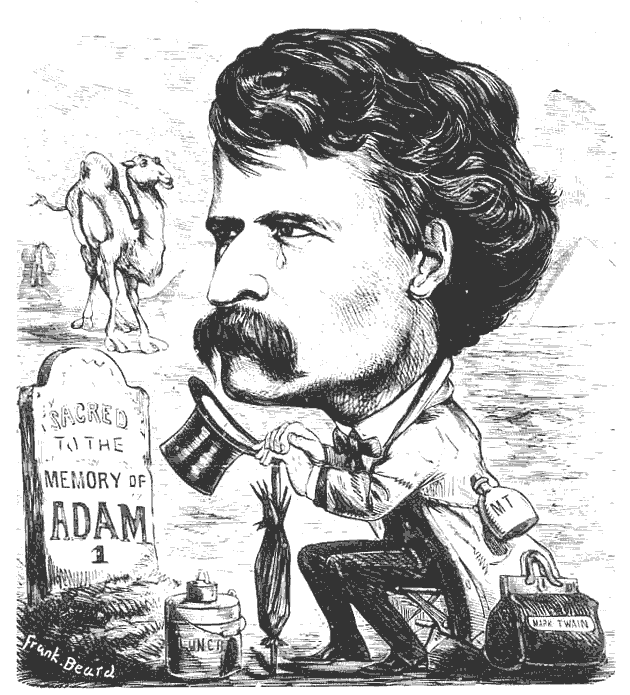
\includegraphics[width=8cm]{img1.png}
	\caption{Ilustração de Frank C.~Beard (\emph{American Publisher}, julho de 1872)}
\end{center}\end{figure}%

\chapter{O contador de histórias Mark Twain}

\begin{flushright}
\textsc{hanna betina gotz}
\end{flushright}
\medskip

\section{Sobre o autor}

\noindent\textsc{Samuel Langhorne Clemens,} o prolífico e famoso escritor conhecido como Mark
Twain, não se tornou uma celebridade da noite para o dia. Passou as três
primeiras décadas de sua vida experimentando trabalhos os mais diversos.
Desde cedo demonstrou pouco interesse pela escola,
pela leitura e a escrita. Apesar de saber soletrar bem --- uma grande
façanha para quem não gosta de estudar ---, a aprendizagem formal, dentro de
quatro paredes, acompanhada de estritas regras de disciplina, o sufocava. Tanto assim que, antes mesmo de
completar doze anos, conseguiu convencer a mãe a deixá"-lo abandonar 
a escola para trabalhar como aprendiz na tipografia do jornal \textit{The Courier},
em Hannibal, Missouri, em troca de roupa e comida. Como a situação
financeira da família era instável, principalmente depois da morte do pai
--- o juiz e comerciante John Clemens ---, a mãe acabou concordando. Aos dezessete
anos, em 1852, já atuava como \textit{journeyman printer} --- um
profissional itinerante de tipografia, que prestava serviços em gráficas
de diversos jornais e, ocasionalmente, escrevia alguma matéria, nem
sempre publicada.

Foi nessa condição, de tipógrafo, que Mark Twain
viu"-se forçado a lidar com o mundo da leitura e da escrita, da reportagem
e da narração de histórias. Até aquele momento, porém, Twain era
apenas Sam, um menino cheio de imaginação e impaciência, que preferia
correr pelas ruas da pequena cidade de Hannibal com outros meninos,
desbravar as encostas dos morros, esconder"-se em cavernas, brincar na
beira do rio Mississippi, pescar, nadar e andar de barco a se submeter a
uma educação formal. Depois de exercer a profissão de tipógrafo e, às
vezes, a de repórter, para jornais em Saint Louis, Nova York e
Filadélfia, e de trabalhar para o jornal de seu irmão Orion, em
Muscatine, Iowa, Sam ainda trabalha como piloto de barco a vapor no
Mississippi, e como minerador --- no promissor e então inexplorado velho oeste,
como correspondente e repórter, e também como soldado, durante a Guerra
Civil, antes de se convencer de que seu verdadeiro talento era o de inventar
histórias. A impressão que se tem é a de que muitas das coisas na vida de
Mark Twain aconteceram por acaso ou por força das circunstâncias.

\section{Sobre a obra}


\subsection{GÊNESE E PUBLICAÇÃO\break DAS SÁTIRAS DA BÍBLIA}

A história da gênese e da publicação dos diários de Adão e Eva é bastante
peculiar e conturbada. Como já foi mencionado, na viagem que
Twain faz à Europa, a bordo do \textit{Quaker City}, começa a ler com entusiasmo
passagens do Velho Testamento. É durante essa viagem que ele visita o lugar de
onde supostamente é retirado o pó, a terra, com que Adão é feito. Também
nessa época, em 1870, três décadas antes de escrever os diários, de dar voz
aos primeiros habitantes da terra, em carta à esposa, Olívia Langdon,
Twain compartilha seu fascínio pela astronomia, pela criação do universo e
a insignificância do ser humano diante da grandeza do infinito:

\begin{quote}
Tenho lido sobre novos argumentos que provam que o mundo é muito antigo \&
que os seus dias de criação foram períodos muito longos. Por exemplo, de
acordo com o livro do Gênesis, as estrelas foram criadas quando o mundo
foi criado, porém este escritor menciona o importante fato de que há
estrelas ao alcance dos nossos telescópios cuja luz precisa de 50 mil anos
para atravessar as imensidões do espaço para chegar à terra. E assim, se
fizermos uma viagem pelo espaço, talvez seja possível, em algum remoto
momento no futuro, que encontremos e cumprimentemos os primeiros raios das
estrelas que começaram sua cansativa viagem de visita a nós há milhares de
anos atrás.

Como somos insignificantes, com o nosso pequeno mundo pigmeu! --- um átomo
reluzindo com incontáveis miríades de outros mundos de átomos, como a lança
de um cavalheiro fluindo do semblante de Deus ---, e ainda assim falamos
complacentemente de nossa manchinha no universo como sendo o Maior dos
Mundos\ldots{} Será que Cristo viveu 33 anos em cada um dos milhões e milhões
de mundos que se mantêm em curso majestosamente sobre nossas cabeças? Ou
será que nosso pequeno globo foi o favorito de todos? Será que uma maçã,
em um grande pomar, pensa sobre si como nós pensamos sobre nós? Será que
as formigas discutem sobre questões polêmicas da teologia da formiga e
será que elas escalam os formigueiros e lançam um olhar sobre o universo
de um acre de terra e dizem: “O Deus que criou tudo isso para nós é bom”?

Não consigo entender como astrônomos se sentem extraordinariamente
insignificantes, pois a cada nova página o Livro dos Céus, que eles
folheiam, revela mais e mais que o mundo do qual somos tão
orgulhosos é, para o universo de globos inclinados, como um mosquito
para os enxames dos alados ou as manadas de animais de casco que
escurecem o ar e habitam as planícies e florestas de toda a terra. Se você
matasse o mosquito, sua falta seria sentida? Honestamente, quem é o
homem para achar que deve ser considerado por Deus? (\textsc{baetzhold} e
\textsc{mccullough}, 1995, p.~xvi)
\end{quote}

\subsection{A CAIXA"-PRETA}

Seu interesse por essa temática era um fato completamente desconhecido de
seus leitores. Graças a um hábito também peculiar de Twain, de guardar
centenas de cartas, documentos, contas, recibos, fotos e, sobretudo,
rascunhos e manuscritos rejeitados por editores em uma espécie de 
caixa"-preta, um velho baú de ``refugos literários''
que chamava de ``Posthumous Box'', é
possível descobrirmos hoje informações como estas, que explicam o que o
motivou a escrever sobre esse assunto e entender o que está por trás do 
\textit{Leitmotiv} dos textos bíblicos: Twain era obcecado pela figura do
personagem Adão. Nesta caixa de material póstumo descobrimos mais uma
informação, de caráter bem cômico, bem típico de Mark Twain, que revela
sua obsessão com o tema da Gênese. Trata"-se de uma história verídica,
relatada por Baetzhold e McCullough. Na caixa havia documentos que relatam
e comprovam os seguintes fatos: em 1879, em Elmira, Nova York, na casa
dos familiares de sua esposa, Olívia, Mark Twain propôs a ideia de erigir
uma estátua de Adão no centro da cidade, uma vez que Adão é “o pai da raça
humana, [e] certamente merece ser honrado” (1995, p.~4). Esta elucubração,
ou delírio, que surgiu primeiramente em tom de brincadeira, ganhou força
a ponto de Twain vir a redigir uma petição ao Congresso americano
para conceder à cidade de Elmira permissão para construir um monumento
a Adão. A petição foi assinada por 94 cidadãos que viram
as possíveis vantagens comerciais e turísticas de tal empreitada. Porém,
ao senador general Joseph Hawley, amigo de Twain, que encaminharia a
petição ao Congresso, ``logo [\ldots{}] surgiram dúvidas sóbrias sobre as
possíveis repercussões [de tal monumento] e devolveu o documento a seu
autor'' (\textsc{idem}, p.~4).

Quando enfim escreve os diários de Adão e Eva, em 1893 e 1905,
respectivamente, não consegue que sejam imediatamente publicados. Não foi à toa
que Twain criou a caixa de material póstumo. Aliás, muitos dos textos que
escrevia, segundo suas próprias palavras, ``[eram] muito
impactantes para o consumo do leitorado'', e só deveriam
tornar"-se públicos cem anos depois de sua morte, condição que impôs
pessoalmente para a publicação do material póstumo, o que significava que ele
poderia falar mais livremente, sem correr riscos, pois adotar uma
persona que falasse da tumba permitia que fosse mais franco (\textsc{quirk},
1994, pp.~vii--xxiv). Os diários de Adão e Eva que temos disponíveis
hoje foram originalmente concebidos e produzidos em duas partes, a
primeira --- ``Fragmentos do diário de Adão'' ---, foi escrita durante a
já mencionada estada da família Clemens na Europa, quando se
hospedam, entre 1892 e 1893, na Villa Viviani, perto de Florença. A segunda
--- ``Diário de Eva'', é escrita quando a família está novamente nos Estados
Unidos, residindo na cidade de Dublin, New Hamsphire, em 1905. Twain submeteu os
``Fragmentos do diário de Adão'' a diversos editores ainda em 1893, mas o
manuscrito foi rejeitado. Graças aos contatos de outrora, em Buffalo, quando
era sócio do \textit{Buffalo Express}, um amigo, então secretário de turismo da
região de Buffalo, sugere que adapte o manuscrito de forma a ambientar o
enredo do mítico Paraíso de Adão e Eva nas cataratas do Niágara, pois
assim poderia ser vendido como souvenir durante a Exposição
Pan"-Americana de Chicago, em 1893. Era uma grande oportunidade de
Divulgar as cataratas para milhares de visitantes do mundo inteiro. Uma das
modificações mais óbvias é aquela em que Eva começa a organizar o Paraíso
colocando placas que indicavam os diversos locais de visitação do lugar,
como se o Jardim do Éden fosse um parque público. No relato Adão diz
que algumas dessas placas indicam: “Por aqui para a piscina de
hidro”, “Por aqui para a ilha das cabras”, “Caverna dos ventos por aqui”
(pp.~6--7).

A segunda parte do diário, ``escrita'' por Eva, é
primeiramente publicada como uma edição especial, natalina, pela revista
\textit{Harper's Bazaar}. Segundo Howard Baetzhold e Joseph Mccullough (1995, p.~
19), o ``Diário de Eva'' pode ter sido uma homenagem póstuma de Twain a Olívia
Langdon, sua esposa, que falecera no ano anterior. Em uma carta ao
cunhado Charles Langdon, ele diz: ``Onde quer que Livy estivesse,
lá era o meu país'' [\textit{Wherever Livy was, that was my country}].
No final do ``Diário de Eva'', o leitor depara com o seguinte
epitáfio em sua tumba, uma homenagem de Adão que revela um sentimento semelhante:
``Onde quer que ela estivesse, lá estava o Éden''. Em 1906, a     
Harper and Brothers decide também publicar o “Diário de Eva” em formato de
livro, com ilustrações de Lester Ralph. Twain aprova as ilustrações
afirmando, em carta ao editor, que:

\begin{quote}
são cheias de graça, charme, inventividade, humor, \textit{páthos}, poesia --- 
são pródigas em mérito. É uma Eva alegre, uma menina doce, inocente e
sedutora, e é tão natural e está tão à vontade no conto como se tivesse acabado de sair dele.
Mas você acha que vestimentas são indispensáveis
para retratar as mulheres?\ldots{} Ela não está maravilhosa no momento em
que corre atrás de Adão e quando sai à procura dele quando ele foge?
Você percebe quão carregada de admiração e interesse pueril ela está?
Roupas vulgarizariam sua imagem --- até mesmo as de uma duquesa.
(\textsc{baetzhold} e \textsc{mccullough}, 1995, p.~18)
\end{quote}

Independente de quão belas eram as ilustrações, elas causaram escândalo, e o
livro foi proibido em algumas bibliotecas, como a Charleton Library de
Worcester, Massachusetts. Twain segue persuadido de que o ``Diário de Eva'' é
uma linda história de amor, ``suave do começo ao fim,
focado nos elementos mais leves e mais divertidos da corte e do
casamento de Adão e Eva'' (\textsc{baetzhold} e \textsc{mccullough}, 1995, p.~19).

As duas partes do diário, em conjunto, são finalmente
publicadas em formato de livro em junho de 1906, pela Harper and Brothers Publishing House. O
desejo do autor, porém, era publicá"-las em sequência com outras obras
da série, de temática afim, como ``That Day In Eden'',
``Eve Speaks'', ``Solilóquio de Adão'',
``Autobiografia de Eva”, “Passagens do diário de Satã'', entre outros.
Isso nunca ocorreu, pelo menos até 1995, quando Baetzhold e McCullough
reuniram e publicaram, na obra intitulada \textit{The Bible According to Mark
Twain}, os mais relevantes textos de temática bíblica encontrados na caixa
póstuma. A partir daí, esses contos --- repletos de sátira, ironia, humor e
certa dose de lirismo --- começam a ser prestigiados em círculos
literários e acadêmicos. Os diários de Adão e Eva, nunca antes incluídos nos
currículos de português"-inglês dos cursos de letras, finalmente ganham a
visibilidade merecida, inclusive no âmbito da dramaturgia, tendo sido
transformados em peça teatral pelo ator e diretor David Birney em meados
dos anos 1990, e em outra produção cênica, pelo diretor Gerald P.~Murphy, 
por volta da virada do século \textsc{xxi}. No Brasil, infelizmente, 
as traduções são escassas, fazendo que a grande maioria de suas obras, 
principalmente as de veia mais satírica, seja conhecida exclusivamente, ou quase,
pelo público que lê Mark Twain diretamente no original. 

\subsection{O DIÁRIO E OUTROS CONTOS\break DE TEMÁTICA BÍBLICA}

A edição de \textit{Diary of Adam and Eve} utilizada nesta tradução pertence à série
A Modern Library Mini, da Modern Library Edition, de 1996, publicada nos
Estados Unidos pela Random House. Está dividida em duas partes: Parte 1 ---
``Fragmentos do diário de Adão'' e Parte 2 --- 
``Diário de Eva'', que vem acrescida de mais
um fragmento do diário de Adão e ainda das seções
``Depois da expulsão'' e ``Quarenta
anos depois'', terminando com o epitáfio na tumba de Eva.

No estilo de um diário, a primeira parte é mantida pelo primeiro
homem judaico"-cristão, Adão. Contado em primeira pessoa, registra os
acontecimentos desde o primeiro dia no Paraíso até a chegada de Eva e as
mudanças que ela institui ali. A segunda parte, contada já por
Eva, a mais nova habitante do Jardim do Éden, descreve o Paraíso e
registra sua perspectiva do comportamento daquele que até então não
tinha nome e que ela decide chamar de Adão. Ela também explica o porquê
das mudanças que faz no ambiente --- a organização e a nomeação das
primeiras coisas, por exemplo, que caracterizam as primeiras tentativas
de comunicação verbal no Paraíso. Neste ponto a história dá um salto de
quarenta anos, quando o casal é expulso do Paraíso. 

Curiosamente, a Parte 2, escrita do ponto de vista de Eva, contém, no
subtítulo, a seguinte observação entre parênteses: “Traduzido do
original”. O que essa observação insinua é que Mark Twain não assume a
autoria da obra, mas sim a tradução. Ou seja, o autor conduz o leitor a
pensar que ele foi “mero” tradutor, e não quem ficcionalizou
propriamente os primeiros acontecimentos narrados no Jardim do Éden.
Se por um acaso do destino a obra vier a ser acusada de blasfêmia, ironia ou
deboche, ou vier a macular o que está no imaginário coletivo, não será Mark
Twain quem terá de se sentar no banco dos réus. Ele apenas traduziu o
texto original. A última subdivisão, escrita por Eva quarenta anos
depois, já longe do Paraíso, é hilária para o leitor atual, por seu estilo
extremamente “meloso”. É visível como Twain vai transformando os
personagens. Se no princípio os dois personagens eram desconhecidos, não
se suportavam pelas óbvias diferenças e a falta de convívio, no final o
texto assume um tom romântico, quase brega e piegas, demonstrando que no
desenrolar da história criou"-se um vínculo emocional e de
cumplicidade muito forte entre eles. Ela ora para que possam “[\ldots{}] passar desta vida juntos 
[\ldots{}] mas se um de nós tiver de ir antes, rogo que seja eu; pois ele
é forte, eu sou fraca, não sou necessária para ele [\ldots{}] a vida sem ele
não seria vida; como eu aguentaria? [\ldots{}]” E no epitáfio de Eva
encontramos o seguinte: “Onde quer que ela estivesse, lá estava o     
Éden”.

O conto intitulado ``Passagens do diário de
Satã'' é finalmente disponibilizado ao público atual, em
língua inglesa, em \textit{The Bible According to Mark Twain}.
A linguagem é bem menos coloquial do que a encontrada nos diários de Adão e
Eva. No momento em que escrevem seus diários, Adão e Eva são ainda muito jovens e
inocentes, e têm dificuldade para expressar suas ideias, até porque são
eles, como expressam nos diários, os responsáveis pelo surgimento da
língua. Já Satã, onipotente, onipresente, como é, se
expressa de forma bem mais sóbria, objetiva e articulada. Nas passagens de
seu diário, Satã relata o teor da conversa que tem com Adão e Eva, quando
casualmente os encontra no Paraíso. Twain retrata um Satã bem
diferente da imagem que habita nosso imaginário coletivo, que na maioria
das vezes é reforçada pela literatura e pelo cinema: a de uma figura
malvada, sádica, sarcástica, que deseja o mal das pessoas, sem dó nem
piedade. O Satã ficcionalizado e reinventado por Twain é
surpreendentemente humano, bondoso e paternal.

A ``Autobiografia de Eva'' assemelha"-se,
parcialmente, ao ``Diário de Eva'', e
constitui a primeira tentativa do autor de escrever sobre Eva no
Paraíso. Os manuscritos datam de 1901 e 1902, enquanto o
``Diário de Eva'' foi escrito em 1905. Segundo
Baetzhold e McCullough, o objetivo de Twain era relacionar as narrativas do
livro do Gênesis ao presente e ao mesmo tempo demonstrar sua teoria
cíclica da história (1995, p.~35). Na “Autobiografia”, além das entradas
diárias e/ou semanais, temos também um olhar retrospectivo, de quando Eva
já está fora do Paraíso. Ela relata em mais minúcias sua relação com Adão
e com os animais, suas experiências científicas e invenções, seu encontro
com Satã, o nascimento dos filhos, o surgimento da língua e sua
preocupação de conseguir expressar"-se através da linguagem. Quem já leu as
passagens do livro do Gênesis e as compara com as narrativas dos diários
de Adão e Eva, da autobiografia dela e dos relatos de Satã se dá conta de que
o dia a dia no Paraíso, longe de ser ideal e perfeito, foi tão atribulado e
humano quanto é o nosso. Nessas narrativas, Twain brinca com a
ideia de que os primeiros habitantes da terra enfrentaram as mesmas
dificuldades e passaram por um processo de aprendizagem, de vitórias e
derrotas, e de construção de sua subjetividade, bastante semelhante ao
nosso. Mas, sobretudo, o que ele mostra através dessa produção tardia é
que o sulista tipógrafo, repórter, soldado, minerador, investidor e
palestrante era, na verdade,

\begin{quote}
um mestre em virtualmente todo
tipo de gênero da prosa; em fábulas e histórias, discursos e ensaios; ele
habilmente adaptava, estendia ou satirizava convenções literárias, guiado
por sua imaginação rebelde (\textsc{quirk}, 1994, quarta capa). 
\end{quote}


\section{Sobre o gênero}
%\section{A IRONIA E A SÁTIRA EM TWAIN}

\begin{quote}
O conto é, do ângulo dramático, unívoco, univalente. [\ldots]
Etimologicamente preso à linguagem teatral,
``drama'' significava ``ação''. E com o tempo passou a designar
toda peça destinada à representação. Na época romântica, dado o
princípio da fusão de gêneros, entendia-se por drama o misto de
tragédia e comédia. Transferido para a prosa de ficção, o termo
``drama'' entrou a significar ``conflito'', ``atrito''. Nesse caso,
``ação'' ``conflito'' se tonaram equivalentes, uma vez que toda
ação pressupõe conflito, e este, promove a ação, ou por meio dela
se manifesta; em suma, ambos se implicam mutuamente.

O conto é, pois, uma narrativa unívoca, univalente: constitui
uma \textit{unidade dramática}, uma \textit{célula dramática}, visto gravitar ao
redor de um só conflito, um só drama, uma só ação. Caracteriza-se,
assim, por conter \textit{unidade de ação}, tomada esta como a sequência de atos praticados pelos protagonistas, ou de acontecimentos de
que participam. A ação pode ser externa, quando as personagens se
deslocam no espaço e no tempo, e interna, quando o conflito se
localiza em sua mente.\footnote{\textsc{moisés}, Massaud. \textit{A criação literária}. São Paulo: Cultrix, 2006, p.\,40.}
\end{quote}

Partindo da definição de Massaud Moisés sobre o conto, evidencia"-se a principal característica desse gênero literário: a unidade de conflito, condensada em ações que se completam em um único enredo. Ao conto, ainda seguindo Moisés, aborrecem as divagações e os excessos, pois há uma concentração de efeitos e pormenores essenciais, em sua brevidade, para o bom funcionamento do conto.
Cada construção, cada palavra nesse gênero tem sua razão de existir, pois integra a economia global da narrativa.

Apesar da brevidade de sua forma, o conto desdobra"-se em muitas direções e implicações, e o faz a partir de elementos restritos: a unidade dramática, como já mencionada, assim como a presença de poucas personagens e a limitação espacial e temporal. No caso de Mark Twain, pode"-se reparar na forte presença da ironia e da sátira em suas narrativas curtas.
A história familiar e pessoal de Twain desvela, em certa medida, o tom satírico do nosso autor.
Diz"-se que do pai, John Clemens, sonhador, visionário, Twain herdou a
falta de habilidade para os negócios. Da mãe, Jane Lampton, forte,
decidida, realista, batalhadora, herdou o senso de humor. Quando nasceu,
ele era tão franzino, raquítico e desengonçado que ninguém pensou que
sobrevivesse. Dos seis irmãos que teve, três morreram antes de alcançar a
puberdade. Mas Twain sobreviveu, talvez por ter nascido com o gene da
obstinação, que, aliás, o acompanhou a vida toda. Segundo a biografia
escrita por Paine, Twain lhe contou que um dia, quando ainda era um menino, a mãe
se queixou ao pequeno Sam, dizendo que vivia assustada, com medo. E ele
perguntou: ``Medo de que eu morra, não é, mamãe?''. ``Não'', disse ela,
``medo de que sobrevivas!'' Essa presença de espírito, essa forma
de humor, de conseguir rir de si mesmo ou das
situações difíceis em que se encontrava, era uma característica materna
que Twain habilmente soube transportar para a literatura e
aplicar na vida pessoal. Nas palestras, nos eventos sociais, nas ruas, na
intimidade da família, era assim que se comportava, sempre tentando
encontrar um jeito de fazer os outros rirem e também rir de si mesmo. E sempre o
fazia daquele mesmo jeito, com cara séria, não deixando ninguém
suspeitar que a próxima frase seria um chiste, algo
engraçado, irônico, debochado ou desconcertante. Como vimos, na infância,
com \textit{uncle} Daniel, o velho escravo da fazenda do tio Quale, aprendera que a
graça ou o interessante das histórias não está nas palavras nem nos fatos
em si, mas em como são ditos, como são contados. Twain não perdia nenhuma
oportunidade para transformar algo que poderia ser considerado uma
tragédia ou desgraça em algo engraçado. É o caso, por exemplo, de quando
ele, na fase de minerador, se tornou milionário. Ele e um de seus
companheiros seguiram uma pista sobre uma mina e a encontraram. Mas, como
não tinham os direitos sobre a exploração, falsificaram a papelada.
Enquanto não foram pegos, foram milionários. Como ele mesmo conta na
abertura de \textit{Roughing it!}, que dedica ao amigo e companheiro de
mineração, o período de milionário durou dez dias:

\begin{quote}
A Calvin H.~Higbie, da Califórnia, homem honesto, camarada genial, amigo de todas as
horas. Este livro foi escrito pelo autor em memória do curioso momento em que
nós dois fomos milionários por dez dias (\textsc{twain}, 1982, p.~692).
\end{quote}

Como insinua a dedicatória, o que ele poderia narrar como um fato
lamentável, trágico, decide narrar como uma história engraçada, hilária,
para ser lembrada para o resto da vida como uma grande piada. Conseguia
transformar, enfeitar e adicionar aos fatos verídicos ingredientes que
sempre tornavam suas histórias em uma \textit{good story} --- uma boa história!

Outro segredo das narrativas twainianas é que ele contava as histórias da
mesma maneira como falava. Twain era conhecido por falar do modo sulista,
com o \textit{southern drawl}, aquele acento carregado, lento, anasalado, sem
pressa, recheado de vocábulos e expressões típicas do sul. Era um
regionalista que não tinha vergonha de sua origem, de suas raízes, nem da
maneira como se falava na região onde cresceu. Twain nunca tentou ser quem não era. Nunca quis passar por pessoa culta,
erudita. E era sempre muito franco a respeito disso e fazia troça daqueles
que considerava ``metidos a besta'', que tentavam passar
por quem não eram. Também no modo de vestir fazia questão de causar
impacto, de não ceder às regras e imposições da classe social mais
elevada, da qual veio a fazer parte, sem se constranger. Na verdade não se
constrangia, mas fazia que os outros se constrangessem, perdessem a
pose. Esse seu comportamento ficava evidente nas palestras, em que
aparecia com o cabelo desgrenhado, sempre com o velho terno de linho
branco, como se tivesse aterrissado ali por engano, por acaso. As folhas
de seu discurso estavam sempre amassadas, fora de ordem, como se fosse um
atrapalhado nato, incurável. Deixava todos desconcertados. E a plateia ria do momento em que ele abria a boca até o final.

Seus famosos aforismos também deixam visível a intenção de dizer a
verdade, de fazer as pessoas perderem a pose rindo, de fazê"-las rir dos
outros até se darem conta de que deveriam rir, ou ter vergonha, de si mesmas.
Seus aforismos fazem o púbico refletir sobre o próprio comportamento,
sobre seu modo possivelmente hipócrita e interesseiro de agir e pensar. Eis
alguns exemplos, retirados de \textit{Mark Twain, Wit and Wisecracks} (1998): 

\begin{itemize}
\item É melhor ficar de boca fechada e parecer um idiota do que abrir a
boca e não deixar nenhuma dúvida.

\item Uma boa criação consiste em ocultar o quanto pensamos sobre nós
mesmos e o quanto desdenhamos os outros.

\item Sejamos gratos aos tolos. Sem eles não teríamos sucesso!

\item Clássico: um livro que as pessoas elogiam, mas ninguém lê.

\item O homem é o único animal que fica ruborizado. Ou que tem motivos para
isso.

\item Tudo o que é humano é patético. O segredo do humor não está na
alegria, mas sim na tristeza. Não há humor no céu.

\item Nada precisa de mais reforma do que os hábitos dos outros.

\item Num primeiro momento Deus fez os idiotas. Só para praticar. Depois
fez os conselhos escolares e os colegiados.

\item Milhares de gênios vivem e morrem sem ser descobertos --- por eles
mesmos ou pelos outros.
\end{itemize}

Um aforismo que nos traz de volta ao tema dos diários de Adão e Eva:
``Adão e Eva tiveram muitas vantagens, mas a principal foi ter
escapado à primeira dentição''.


